\documentclass[compress]{beamer}

\usepackage[nofonts]{ctex}
\setCJKmainfont[ItalicFont={Kaiti SC}]{Kaiti SC}
%\setCJKmainfont[ItalicFont={AR PL KaitiM GB}]{AR PL KaitiM GB}%
%\setCJKsansfont{WenQuanYi Zen Hei}% 文泉驿的黑体


\mode<beamer>
{
    \useinnertheme{rounded}
    \useoutertheme{split}
    \usecolortheme{rose}
    \usecolortheme{seahorse}
}

\mode<handout>
{
	\usetheme{default}
	\usepackage{pgfpages}
	\pgfpagesuselayout{4 on 1}[a4paper,landscape,border shrink=5mm]
}


\usepackage{amsmath,latexsym,amssymb,amsfonts,amsbsy}
\usepackage{graphicx}
\usepackage{hyperref}
\usepackage{listings}
\usepackage{fancyvrb}
\fvset{frame=single,fontsize=\small}

\newcommand{\romannumber}[1]{{\textrm{\uppercase\expandafter{\romannumeral
#1}}}}

\setbeamercolor{dblue}{fg=white,bg=blue!40!gray} % for beamercolorbox
\newenvironment{pblock}{\begin{beamercolorbox}[rounded=true,
      shadow=true]{dblue}}{\end{beamercolorbox}}


\graphicspath{{figure/}}

\lstset{
	basicstyle=\footnotesize, % print whole listing footnotesize
	keywordstyle=\footnotesize\color{black}\bfseries, 
	identifierstyle=\footnotesize\color{blue}, 
	commentstyle=\footnotesize\itshape, 
	stringstyle=\footnotesize\ttfamily,
	frame=single, 
	numbers=left, numberstyle=\tiny,
	stepnumber=1, numbersep=10pt,
	showtabs=false, tabsize=4,
	showstringspaces=false,
	breaklines=true, breakatwhitespace=true,
	language=[ISO]C++
}   


%%%%%%%%%%%%%%%%%%%%%%%%%%%%%%%%%%%%%%%%%%%%%%%%%%%%%%%%%%%%%%%%%
%    body                                                       %
%%%%%%%%%%%%%%%%%%%%%%%%%%%%%%%%%%%%%%%%%%%%%%%%%%%%%%%%%%%%%%%%%


\begin{document}

\AtBeginSection[]
{ 
    \begin{frame}<beamer> 
		\frametitle{内容提要} 
		\tableofcontents[currentsection,currentsubsection] 
	\end{frame} 
} 
					
\title{开源软件开发}

\author[\href{http://c.pku.edu.cn/}{http://c.pku.edu.cn/}]
{曹东刚\\\href{mailto:caodg@sei.pku.edu.cn}{caodg@sei.pku.edu.cn}}

\institute{Linux程序设计环境 \\
\href{http://c.pku.edu.cn/}{
http://c.pku.edu.cn/}}

\date{}

\titlegraphic{
\includegraphics[height=0.17\textwidth]{Overlays/logo.pdf}}

\begin{frame}
	\titlepage
\end{frame}

\section{开源软件}

\begin{frame}
\frametitle{软件分类}
\begin{itemize}
\item 商业软件 (Business Software/Commercial Software)
\item 共享软件 (Shareware)
\item 公有软件 (Public Domain Software)
\item 自由软件 (Free Software, Open-source Software)
\end{itemize}


\end{frame}

\begin{frame}
\frametitle{自由软件}
\begin{block}{自由软件是一种版权法意义上的定义}
体现在软件知识产权保护层面上. 使用者可以
\begin{itemize}
\item 可以自由使用该软件, 无论出于何种目的
\item 自由学习该程序怎样工作, 并使之适应被许可人的需求
\item 可以自由重新分发、复制以便帮助亲友
\item 可以自由改善该程序,并发布给公众, 让整个社会得利
\end{itemize}
\end{block}

\end{frame}

\begin{frame}
\frametitle{自由软件 vs 开放源码软件}
\begin{itemize}
\item 定义角度不同
    \begin{itemize}
    \item 开源软件: 技术层面
    \item 自由软件: 被许可的权利层面
    \end{itemize}
\item 许可证中对被许可人权利限制的严格程度不同
    \begin{itemize}
    \item 开源软件: 稍宽
    \item 自由软件: 严格
    \end{itemize}
\item 另一种说法为: 自由软件专指遵守GPL的软件, 自由软件包含于开源软件范畴
\end{itemize}


\end{frame}

\begin{frame}
\frametitle{开源软件的认定机构}
OSIA: Open Source Initiative Association\footnote{\href{http://www.opensource.org}{http://www.opensource.org}}
\begin{itemize}
\item Eric S. Raymond等人1998年成立的非营利性组织
\item 将OSI申请为证明商标(OSI Certified)
\item 将OSI商标许可给经审核认定为开源软件的软件提供者
\item 开源软件许可证都可以标明OSI商标, 从而得到开源社区认可
\item 目前有50多个许可证
\end{itemize}
\end{frame}

\begin{frame}
\frametitle{开源软件及许可证的认定标准--1}
\begin{itemize}
\item Free Redistribution(自由发布)
\item Source Code(对源代码的要求)
\item Derived Works(演绎作品)
\item Integrity of The Author's Source Code(保持源代码的完整性)
\item No Discrimination Against Persons or Groups(不得歧视任何个人或团体)

\end{itemize}

\end{frame}

\begin{frame}
\frametitle{开源软件及许可证的认定标准--2}
\begin{itemize}
\item No Discrimination Against Fields of Endeavor(不得歧视任何应用领域)
\item Distribution of License(许可证的发布)
\item License Must Not Be Specific to a Product(不得限制许可协议专属于某一个软件)
\item License Must Not Restrict Other Software(许可证不能影响其他软件)
\item License Must Be Technology-Neutral(许可证应保持技术中立性)
\end{itemize}

\end{frame}


\begin{frame}
\frametitle{开源软件的著作权分析 ---1 }
\begin{itemize}
\item 开放源码软件受著作权保护
\item 开放源码软件作者并没有放弃任何权利, 只是有条件的将某些权利授予所有愿意接受条件的人
\item 被许可人只有在发布了软件的修改版本或演绎作品时才承担相应的义务
\item 开放源码软件受著作权保护
  \end{itemize}
  
\end{frame}

\begin{frame}
\frametitle{开源软件的著作权分析 ---2 }
\begin{itemize}
\item 演绎作品问题
    \begin{itemize}
      \item 演绎权: 改编、翻译、整理、注释、编辑
      \item 对开放源码软件进行演绎, 必须获得原始著作权人的许可
      \item 各种开源软件许可证之间的最大区别往往体现在对演绎作品的态度
    \end{itemize}
\end{itemize}

\end{frame}

\section{开源许可证}

\begin{frame}
\frametitle{开源许可证的共同点}
\begin{itemize}
\item 承认版权
\item 发布的义务---将获得的源代码再发布
\item 对发布的源代码的要求---须保证源代码的完整和可以被获得
\item 允许修改---可以根据获得的源代码产生演绎作品
\item 没有担保
\end{itemize}

\end{frame}

\begin{frame}
\frametitle{开源软件许可证的不同点}
\begin{itemize}
\item 是否允许同其他非开源软件代码混合
\item 是否必须公开修改后的程序
\item 是否明确了专利许可授权
\item 是否明确了专利侵权诉讼导致许可证协议终止
\item 是否明确允许与函数库连接
\item 是否只能按本许可证发布源代码
\item 是否要求对于获得的源代码可能存在知识产权问题进行明确提示
\end{itemize}


\end{frame}

\begin{frame}
\frametitle{开源软件许可证的比较}

{\tiny
\begin{tabular}{|p{0.8cm}|p{1cm}|p{1cm}|p{1cm}|p{1cm}|p{1cm}|p{1cm}|p{1cm}|}\hline
不同点对比 & 是否允许同非开源软件代码混合 & 是否可以将对源代码的修改不公开
& 是否明确了专利许可授权 & 是否明确了专利侵权诉讼导致许可证协议终止
& 是否明确禁止与函数库连接 & 是否只能按本许可证发布源代码
& 是否要求对源代码可能存在的知识产权问题明确提示 \\ \hline
GPL & $\times$ & $\times$ & $\times$ & $\times$ & $\surd$ & $\surd$ & $\times$ \\ \hline
LGPL & $\surd$ & $\times$ & $\times$ & $\times$ & $\times$ & $\times$ & $\times$ \\ \hline
BSD & $\surd$ & $\surd$ & $\times$ & $\times$ & $\times$ & $\times$ & $\times$ \\ \hline
MPL & $\surd$ & $\surd$ & $\times$ & $\times$ & $\times$ & $\times$ & $\times$ \\ \hline
Apache & $\surd$ & $\surd$ & $\times$ & $\times$ & $\times$ & $\times$ & $\times$ \\ \hline
Artistic & $\surd$ & $\surd$ & $\surd$ & $\surd$ & $\times$ & $\times$ & $\times$ \\ \hline
\end{tabular}}

\end{frame}

\begin{frame}
\frametitle{MIT或 X Consortium}
最宽松的许可证
\begin{itemize}
\item 在所有修改版本中保留版权和许可证条款
\item 无限制的复制、使用、修改和再发行
\end{itemize}

\end{frame}

\begin{frame}[fragile]
\frametitle{MIT许可 示例}
\scriptsize
\begin{verbatim}
Copyright (c) 1898-2012 Peking University

Permission is hereby granted, free of charge, to any person obtaining a 
copy of this software and associated documentation files (the "Software"), 
to deal in the Software without restriction, including without limitation 
the rights to use, copy, modify, merge, publish, distribute, sublicense, 
and/or sell copies of the Software, and to permit persons to whom the 
Software is furnished to do so, subject to the following conditions:

The above copyright notice and this permission notice shall be included in 
all copies or substantial portions of the Software.
\end{verbatim}
\end{frame}

\begin{frame}[fragile]
\frametitle{MIT许可 示例 (cont.)}
\scriptsize
\begin{verbatim}
THE SOFTWARE IS PROVIDED "AS IS", WITHOUT WARRANTY OF ANY KIND, EXPRESS OR 
IMPLIED, INCLUDING BUT NOT LIMITED TO THE WARRANTIES OF MERCHANTABILITY, 
FITNESS FOR A PARTICULAR PURPOSE AND NONINFRINGEMENT. IN NO EVENT SHALL THE
AUTHORS OR COPYRIGHT HOLDERS BE LIABLE FOR ANY CLAIM, DAMAGES OR OTHER 
LIABILITY, WHETHER IN AN ACTION OF CONTRACT, TORT OR OTHERWISE, ARISING 
FROM, OUT OF OR IN CONNECTION WITH THE SOFTWARE OR THE USE OR OTHER 
DEALINGS IN THE SOFTWARE.
\end{verbatim}

\end{frame}


\begin{frame}
\frametitle{BSD}
比MIT稍微严格. 最先用于BSD 4.4版本上, 现被Apache和BSD操作系统等开源软件采纳。
\begin{itemize}
\item 在所有修改版本中保留版权和许可证条款, 并在广告和软件包相关文档中包含对所有程序开发者的致谢
\item 无限制的复制、使用、修改和再发行
\end{itemize}
最新的BSD许可证删除了对广告的要求, 实际上等价于MIT许可证

\end{frame}

\begin{frame}[fragile]
    \frametitle{新BSD许可示例} 
{
\scriptsize
\begin{verbatim}
Copyright (c) 2010, Peking University (PKU).
All rights reserved.

Redistribution and use in source and binary forms, with or without
modification, are permitted provided that the following conditions
are met:
1. Redistributions of source code must retain the above copyright
   notice, this list of conditions and the following disclaimer.
2. Redistributions in binary form must reproduce the above copyright
   notice, this list of conditions and the following disclaimer in
   the documentation and/or other materials provided with the distribution.
3. Neither the name of the PKU nor the names of its contributors may be 
   used to endorse or promote products derived from this software without 
   specific prior written permission.
\end{verbatim}
}
\end{frame}

\begin{frame}[fragile]
    \frametitle{新BSD版权声明示例 (cont.)} 
{
\scriptsize
\begin{verbatim}
THIS SOFTWARE IS PROVIDED BY THE REGENTS AND CONTRIBUTORS ``AS IS'' AND
ANY EXPRESS OR IMPLIED WARRANTIES, INCLUDING, BUT NOT LIMITED TO, THE
IMPLIED WARRANTIES OF MERCHANTABILITY AND FITNESS FOR A PARTICULAR PURPOSE
ARE DISCLAIMED.  IN NO EVENT SHALL THE REGENTS OR CONTRIBUTORS BE LIABLE
FOR ANY DIRECT, INDIRECT, INCIDENTAL, SPECIAL, EXEMPLARY, OR CONSEQUENTIAL
DAMAGES (INCLUDING, BUT NOT LIMITED TO, PROCUREMENT OF SUBSTITUTE GOODS
OR SERVICES; LOSS OF USE, DATA, OR PROFITS; OR BUSINESS INTERRUPTION)
HOWEVER CAUSED AND ON ANY THEORY OF LIABILITY, WHETHER IN CONTRACT, STRICT
LIABILITY, OR TORT (INCLUDING NEGLIGENCE OR OTHERWISE) ARISING IN ANY WAY
OUT OF THE USE OF THIS SOFTWARE, EVEN IF ADVISED OF THE POSSIBILITY OF
SUCH DAMAGE.
\end{verbatim}
}
\end{frame}

\begin{frame}
\frametitle{MPL: The Mozilla Public License}
\begin{itemize}
\item 允许将别人的源代码用于自己的商业行为
    \begin{itemize}
      \item 在自己的源代码库上加一个接口, 除了接口程序的源代码以MPL许可发布, 源代码库中的源代码不必用MPL许可对外发布
    \end{itemize}

\item 可与其他类型的代码混合得到自己的软件
\item 源码提供者不能提供受专利保护的源码, 也不能在将代码以开源许可证许可后再申请专利
\item 对修改的源代码以网络形式发布有时间上的要求: 网页保留至少12个月
\end{itemize}
\end{frame}


\begin{frame}
\frametitle{GPL: General Public License}
\begin{itemize}
\item 自由软件联盟 GNU的开源软件许可证的一种
\item 开源软件领域最富盛名
\item 对被许可人权利限制最严
\item 最大限度保证软件自由
\end{itemize}

GPL的理念: 在承认版权的前提下, 通过软件的版权许可来实现自由软件的自由权利的要求
\begin{itemize}
\item 复制权、发行权、修改权、翻译权
\end{itemize}


\end{frame}

\begin{frame}
\frametitle{GPL的传染性}

\begin{itemize}
\item 凡是在逻辑上与GPL软件相联系并作为整体发布的程序中,
只要有任何一部分代码是以GPL发布的, 那么全部程序作为整体就必须接受GPL的约束
\item 适用于GPL的程序代码, 包括该程序以及由该程序衍生出来的``基于程序的作品''

\end{itemize}


\end{frame}

\begin{frame}
\frametitle{GPL被许可人的义务---1}
\begin{itemize}
\item 声明: 版权声明, 免责声明, 保证声明完整无损
\item 修改说明: 在修改的文件中附有明确的修改说明以及具体日期
\item 传递GPL条款: 当被许可人发布或出版作品时, 必须遵照GPL条款作为整体全部免费许可给任何第三方
\end{itemize}


\end{frame}

\begin{frame}
\frametitle{GPL被许可人的义务---2}
\begin{itemize}
\item 必要的提示: 交互式程序运行前打印声明
\item 发布时提供源代码
\item 被许可人没有再许可的权利与义务: 从原始著作人处获得权利
\item 无担保和免责条款: 非强制性
\end{itemize}


\end{frame}

\begin{frame}
\frametitle{GPL当事人及其关系的确定}

\begin{itemize}
\item GPL许可证的一方当事人始终是``原始许可证颁布者'', 即首先发布受GPL保护的程序的人
\item GPL许可证的另一方当事人是程序的下游被许可人, 他们无差别的享有原始发布者赋予的权利和承担相同的义务
\end{itemize}

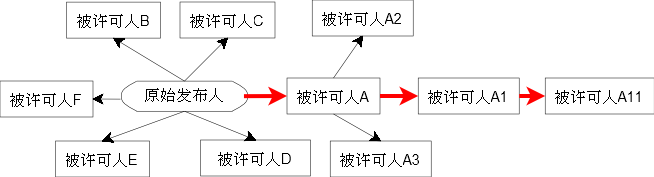
\includegraphics[width=1.0\hsize]{gpled.png}


\end{frame}

\begin{frame}
\frametitle{LGPL: Lesser General Public License}

主要针对函数库类型软件
\begin{itemize}
\item 允许其它应用程序与库进行连接
\item 区分了``基于函数库的作品''与``使用函数库的作品''
    \begin{itemize}
    \item 前者包含来自函数库修改过的源代码
    \item 后者必须与函数库结合才能执行
    \end{itemize}
\item 对于选用LGPL许可证公开的源代码, 可以变更为适用GPL许可证; 但不能反向变更
\end{itemize}


\end{frame}


\begin{frame}
\frametitle{开源软件的侵权纠纷}
\begin{itemize}
\item 侵犯OSIA及许可人的商标权
\item 发布不享有版权的软件产生的版权纠纷
\item 发布侵犯他人专利权产生的专利权纠纷
\end{itemize}

\end{frame}

\begin{frame}
\frametitle{开源软件的违约纠纷}

\begin{itemize}
\item 发布软件时未标明版权信息及必要的修改信息
\item 发布软件时没有附上相应的许可证
\item 源代码的提供不符合许可证的要求
\item 违反许可证的规定将软件代码与其他代码混合
\item 发布软件时违反许可证规定收取不适当的费用
\item 违反许可证的规定以开源软件申请专利
\item 许可证间的冲突带来的违约行为
\end{itemize}

\end{frame}

\begin{frame}
\frametitle{开放源码司法案例: SCO vs IBM vs Novell}
\begin{itemize}
\item 2003年3月美国犹他州盐湖城法院, SCO诉IBM侵权Unix,后相继起诉Novell, AutoZone, DaimlerChrysler
\item SCO警告财富榜1000, 全球500强, 全部Linux用户(赔偿1399\$/处理器)
\item IBM和Red Hat公司反诉讼
\item SCO将Unix代码授权给微软
\item SCO变换指控, 案情越来越复杂
\item 2006, 法官驳回SCO的294条主张中的182条
\item 2007和2010, 法院两次判决Novell是Unix版权拥有者
\item SCO 破产,Nasdaq 摘牌
\end{itemize}
\end{frame}

\begin{frame}
\frametitle{SCO vs IBM vs Novell: Unix版权}
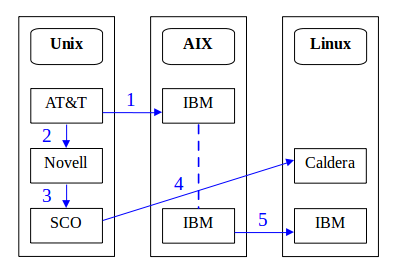
\includegraphics[scale=0.5]{unix_right.png}
\end{frame}

\begin{frame}
\frametitle{自由和开源社区的反应}
\begin{itemize}
\item SCO甚至并不拥有那些有争议的源码
\item Linux不大可能会有Unix的代码
\item Linux采用SCO UNIX代码无意义
\item 即使Linux和SCO UNIX某代码相似, 也并不能证明其来源于SCO
\item SCO之前是Linux厂商, 可能从Linux复制了代码
\item 即使Linux从SCO复制了代码, 但SCO UNIX代码之前已经在没有保密约定的情况广泛传播了, 不存在商业泄密问题
\item 即使Linux有UNIX代码, SCO也没权利以泄漏商业秘密或侵权为由起诉IBM
\end{itemize}
\end{frame}

\begin{frame}
\frametitle{案件背后的问题}
\begin{itemize}
\item GPL的法律效力
\item 开源软件代码规范性
\item 版权陷阱
\item 专利威胁
\item 商业化
\item 自主知识产权
\end{itemize}

\end{frame}


\section{开源软件开发实践}

\begin{frame}
\frametitle{开源软件开发的规则 ---1}
\begin{itemize}
\item 源码公开
    \begin{itemize}
    \item 代码和过程公开, 鼓励同行复审
    \end{itemize}
\item 尽早发布, 经常发布
    \begin{itemize}
    \item 确保第一次发布能编译和运行, 实现了承诺的功能
    \item 缩短和加速用户与开发者之间的反馈
    \end{itemize}
\end{itemize}


\end{frame}
\begin{frame}

\frametitle{开源软件开发的规则 ---2}
\begin{itemize}
\item 对贡献者致谢并表扬
    \begin{itemize}
    \item 即使有物质奖励, 也别忘了精神表扬
    \item 核心团队特权最小化
    \end{itemize}
\item 遵循Unix尽可能自动化的传统
\end{itemize}


\end{frame}

\begin{frame}
\frametitle{协同开发的最佳实践}
\begin{pblock}
开源软件开发的最佳实践实际上就是分布式协同开发实践
\end{pblock}
\begin{itemize}
\item 良好的修补实践
\item 良好的项目命名实践
\item 良好的开发实践
\item 良好的发行制作实践
\item 良好的交流实践
\end{itemize}

\end{frame}

\begin{frame}
\frametitle{良好的修补实践--1}
\begin{itemize}
\item 发送补丁而不是完整的档案包或文件
    \begin{itemize}
    \item 接受补丁的开发者可能已经更改了主干版本
    \item diff文件节省时间
    \end{itemize}
\item 如果补丁被拒绝, 不要太在意
\item 发送针对当前版本代码的补丁
    \begin{itemize}
    \item 补丁提交者应当跟踪主干代码库
    \end{itemize}

\end{itemize}

\end{frame}

\begin{frame}[fragile]
\frametitle{良好的修补实践--2}
\begin{itemize}
\item 不包含可生成文件的补丁
    \begin{itemize}
    \item 如Bison或Flex产生的C文件, 以及autoconf产生的configure脚本
    \end{itemize}
\item 使用\verb~-c或者-u~格式的diff文件
    \begin{itemize}
    \item 缺省的diff输出(\verb~-e~)不包含上下文, 非常脆弱
    \end{itemize}

\item 在补丁中包含手册页和其它文档文件
    \begin{itemize}
    \item 尤其是补丁增加了用户接口部分或改变了软件功能特征
    \end{itemize}
\end{itemize}


\end{frame}

\begin{frame}
\frametitle{良好的修补实践--3}
\begin{itemize}
\item 在补丁中包含解释(告诉维护者)
    \begin{itemize}
    \item 谦逊而自信地说明为什么补丁是必须和有用的, 例如:\\
    ``This patch solves the immediate problem,
    but I realize it complicates the memory allocation in an unpleasant way.
    Works for me, but you should probably test it under heavy load before shipping''
    \end{itemize}

\end{itemize}


\end{frame}

\begin{frame}[fragile]
\frametitle{良好的修补实践--4}
\begin{itemize}

\item 在代码中包含有用的注释
    \begin{itemize}
    \item 糟糕的注释: \\
    \verb~/* norman newbie fixed this 13 Aug 2001 */~
    \item 良好的注释:
	  {\small
\begin{Verbatim}
/*
 * This conditional needs to be guarded so that
 * crunch_data() never gets passed a NULL pointer.
 * <norman_newbie@foosite.com>
 */
\end{Verbatim}
}

    \end{itemize}
\end{itemize}


\end{frame}

\begin{frame}
\frametitle{良好的命名实践--1}
\noindent GNU风格命名法: 主干 + major.minor.patch的编号法
  {\small
    \begin{enumerate}
    \item project prefix (全小写, 只包含字母和数字)
    \item dash
    \item version number
    \item dot
    \item ``src'' or ``bin'' (optional)
    \item dot
    \item binary type and options (optional)
    \item archiving and compression extensions
    \end{enumerate}
	}

\end{frame}

\begin{frame}[fragile]
\frametitle{GNU命名示例}
\noindent 一个叫``foobar''的项目, 主版本号1, 次版本号2, 补丁级别3, 则\\
\begin{tabular}{p{6cm}l}
foobar-1.2.3.tar.gz & $\surd$ \\
foobar123.tar.gz & $\times$ \\
foobar1.2.3.tar.gz & $\times$ \\
foobar-v1.2.3.tar.gz & $\times$ \\
\verb~foo_bar-1.2.3.tar.gz~ & $\times$ \\
FooBar-1.2.3.tar.gz & $\times$ \\
foobar-1.2.3.bin.i386.tar.gz & $\surd$ \\
\end{tabular}

\end{frame}

\begin{frame}[fragile]
\frametitle{良好的命名实践--2}

\begin{itemize}
  \item 采用适合计算机程序可以解析和理解的规则模式
\item 尊重适当的本地项目和社区的约定
    \begin{itemize}
    \item 例如, Apache的模块命名: \verb~mod_foo~ 合法
    \end{itemize}
\item 选择一个唯一的、容易读写和记忆的项目名称.\\
到下述站点作名称搜索
    \begin{description}
    \item ibiblio: \href{http://www.ibiblio.org/pub/Linux/}{http://www.ibiblio.org/pub/Linux/}
    \item freshmeat: \href{http://www.freshmeat.net}{http://www.freshmeat.net}
    \item sourceforge: \href{http://www.sourceforge.net}{http://www.sourceforge.net}
    \end{description}

\end{itemize}

\end{frame}

\begin{frame}[fragile]
\frametitle{良好的开发实践--1}
\begin{itemize}
\item 不依赖专有语言、函数库或其他代码
    \begin{itemize}
    \item 开源开发者不相信他们无法评审的源码
    \end{itemize}
\item 使用GNU自动工具处理移植性问题\\
\verb~configure; make; make test; make install~
    \begin{itemize}
    \item 使用\alert{autoconf}, \alert{autoheader} 或\alert{automake}
    \item 安装软件时尽可能少地向系统询问配置信息
    \end{itemize}
\end{itemize}


\end{frame}

\begin{frame}
\frametitle{好的开发实践--2}
\begin{itemize}
\item 先测试再发布代码
    \begin{itemize}
    \item 建立强大易用的测试框架, 便于进行回归测试
    \item 将测试用例(test suite)和代码一起发布
    \end{itemize}
\item 代码发布前进行健全检查, 清除易忽略的错误
    \begin{itemize}
    \item 用\alert{gcc}编译C/C++程序时打开-Wall选项, 清除所有的警告
    \item 使用查找内存泄露和运行时刻错误的软件, 如 Electric Fence和Valgrind
    \end{itemize}

\end{itemize}


\end{frame}

\begin{frame}[fragile]
\frametitle{好的开发实践--3}

\begin{itemize}
\item 发布前对文档和README进行拼写检查
\item C/C++移植性实践
    \begin{itemize}
    \item 对C语言应完全使用ANSI功能特征
    \item 不使用编译器的专门特征
    \item 需要移植的代码被隔离在一个单独区域(如 os 子目录), 创造一个分离的移植层
    \item 在移植层外尽量少用\verb~#ifdef和#if~
    \item 选择并严格坚持一个编码规范
    \end{itemize}
\end{itemize}


\end{frame}

\begin{frame}[fragile]
\frametitle{良好的制作发行实践--1}
\begin{itemize}
\item 遵从标准的文件命名实践
\item 确保打包文件总是解包到一个单一的新目录下\\
例: \verb~foo-0.23.tar.gz~的文件包应该解压到\verb~foo-0.23~目录
\item 为可升级性设计
    \begin{itemize}
    \item 考虑支持多个软件版本在同一系统中共存, 尤其是库
    \end{itemize}
\end{itemize}


\end{frame}

\begin{frame}
\frametitle{良好的制作发行实践--2}
\begin{itemize}
  \item 项目根目录下包含如下文件\\
\begin{tabular}{p{3cm}l}
README & 最先被阅读的重要文件 \\
INSTALL & 配置、编译和安装向导 \\
HISTORY & 项目历史 \\
COPYING & 项目许可证条款(GNU惯例) \\
FAQ & 项目常见问题解答的纯文本文档 \\
AUTHORS & 项目贡献者列表(GNU惯例) \\
NEWS & 最近的项目新闻 \\
CHANGES & 修订版本之间重大更改的日志 \\

\end{tabular}
\end{itemize}


\end{frame}

\begin{frame}
\frametitle{良好的制作发行实践--3}
\noindent REDAME文件应该短小精悍, 包含:
{\small
  \begin{enumerate}
    \item 项目的简短描述
    \item 指向项目站点的WEB链接, 项目邮件列表地址
    \item 开发者编译环境的注意事项以及潜在的移植性问题
    \item 重要文件和子目录的描述
    \item 项目贡献者的列表
    \item 编译/安装指令或指向同样内容的文件(INSTALL文件)
    \item 项目的最近新闻或指向同样内容的文件(NEWS文件)
  \end{enumerate}
  }
	
  \end{frame}

\begin{frame}
\frametitle{良好的制作发行实践--4}
\begin{itemize}
\item 为Linux提供RPM, deb等预安装包
    \begin{itemize}
    \item 由Makefile自动生成
    \end{itemize}
\item 提供二进制文件的校验和, 允许人们验证文件和正确性
    \begin{itemize}
    \item 可用命令: \alert{sum}, \alert{cksum}, \alert{md5sum}, \alert{gpg}
    \item 在项目网页上列出发布的二进制文件的校验和及其生成命令
    \end{itemize}
\end{itemize}


\end{frame}

\begin{frame}
\frametitle{良好的交流实践--1}
\begin{itemize}
\item 在freshmeat上或主题新闻组(usenet)发布通告\\
通告应该言简意赅, 说明软件的目的
\item 建立项目网站, 至少包含如下内容
    \begin{itemize}
    \item 项目说明(项目建立的理由, 面向的群体等)
    \item 项目源码/二进制码的下载链接
    \item 如何加入项目邮件列表的指导
    \item 常见问题回答列表 (FAQ)
    \item 项目文档的HTML版本
    \item 相关或竞争项目的链接
    \end{itemize}
\end{itemize}


\end{frame}

\begin{frame}
\frametitle{良好的交流实践--2}
\begin{itemize}
\item 提供项目邮件列表. 对于项目foo
    \begin{itemize}
    \item 私有的开发者列表: foo-dev@mail.domain
    \item 公开的通告列表: foo-announce@mail.domain
    \end{itemize}
\item 发布到主要的档案站点
    \begin{itemize}
    \item ibiblio: \href{http://www.ibiblio.org/pub/Linux/}{http://www.ibiblio.org/pub/Linux/}
    \item freshmeat: \href{http://www.freshmeat.net}{http://www.freshmeat.net}
    \item sourceforge: \href{http://www.sourceforge.net}{http://www.sourceforge.net}
    \item 专门站点
    \end{itemize}
\end{itemize}

\end{frame}

\begin{frame}
\frametitle{选择合适的许可证}
\begin{itemize}
\item 发布于公共域, 无许可证
\item MIT或X Consortium许可证
\item BSD许可证
\item Artistic许可证
\item GNU GPL和LGPL许可证
\item Mozilla公共许可证
\item Apache许可证
\end{itemize}

\end{frame}

\end{document}
